% Copyright (c) 2005-2008 Center for Urban Simulation and Policy Analysis,
% University of Washington.  Permission is granted to copy, distribute and/or
% modify this document under the terms of the GNU Free Documentation License,
% Version 1.2 or any later version published by the Free Software Foundation;
% with no Invariant Sections, no Front-Cover Texts, and no Back-Cover Texts.
% A copy of the license is included in the section entitled "GNU Free
% Documentation License".

\section{Example of Using Datasets, Storage and Variables}
\label{opus-core-dataset-tutorial}

As described in Section~\ref{sec:opus-core-datasets}, a dataset \datasetindex in Opus is considered 
as a $n \times m$ table where $n$ is the
number of entries and $m$ is the number of characteristics, \characteristicsindex also called
attributes. \attributesindex One of the characteristics \characteristicsindex must have unique values
that are numeric larger than 0.

Suppose you have a set of household agents \index{household agents} with two characteristics, \characteristicsindex income
and number of persons per household, which are uniquely identified by
household IDs. The file \file{data/examples/households.tab} in the \package{opus_core}
package contains an example dataset \datasetindex for 10 households:
\begin{verbatim}
household_id   income         persons
 1               1000           2
 2               2000           3
 3               5000           3
 4               3000           2
 5                500           1
 6              10000           4
 7               8000           4
 8               1000           1
 9               3000           2
10              15000           5
\end{verbatim}

Datasets are independent from the physical storage of the data. A data storage
is represented by a python object, specifically, an instance of class \class{Storage} (see Section~\ref{sec:data-storage}). 
We create a storage object for the ASCII file \file{households.tab}:

 \label{storagepage}
\begin{verbatim}
>>> import os
>>> import opus_core
>>> oc_path = opus_core.__path__[0]
>>> from opus_core.storage_factory import StorageFactory
>>> storage = StorageFactory().get_storage('tab_storage',
        storage_location = os.path.join(oc_path, 'data/examples'))
\end{verbatim}

Now we can create a household dataset:
\begin{verbatim}
>>> from opus_core.datasets.dataset import Dataset
>>> households = Dataset(in_storage = storage,
                         in_table_name = 'households', 
                         id_name='household_id',
                         dataset_name='household')
\end{verbatim}

\class{Dataset} supports lazy loading. Thus, there are no entries
loaded for \verb|households| at this moment:
\begin{verbatim}
>>> households.get_attribute_names()
[]
\end{verbatim}
But the dataset \datasetindex `knows' about attributes \attributesindex living on the given storage:
\begin{verbatim}
>>> households.get_primary_attribute_names()
['household_id', 'income', 'persons']
\end{verbatim}
The data are loaded as they are needed. For example, loading the
unique identifier of the dataset \datasetindex gives:
\begin{verbatim}
>>> households.get_id_attribute()
array([ 1,  2,  3,  4,  5,  6,  7,  8,  9, 10])
>>> households.size()
10
\end{verbatim}

Other attributes \attributesindex can be loaded via the \method{get_attribute()} \attributesindex method which
returns a numpy array:
\begin{verbatim}
>>> households.get_attribute("income")
array([  1000.,   2000.,   5000.,   3000.,    500.,  10000.,   8000.,
         1000.,   3000.,  15000.])
>>> households.get_attribute_names()
['household_id', 'income']
\end{verbatim}

Each attribute \attributesindex of a \class{Dataset} is stored as a numpy array. \numpyindex

In the above example, each of the attributes \attributesindex is
loaded separately. Alternatively, we can load multiple attributes
\attributesindex at once, which can be useful when loading data from
a slow storage, such as a SQL database:
\begin{verbatim}
>>> households.load_dataset()
>>> households.get_attribute_names()
['household_id', 'persons', 'income']
\end{verbatim}
An optional argument \verb|attributes| can be passed to the \method{load_dataset()}
method that specifies names of attributes \attributesindex to be loaded, e.g. \verb|attributes=['income', 'persons']|.

% The character "'" does comes out as a right-single-quote, not a vertical-
% quote, which makes it fail when copy-pasting from Acrobat to a Python shell.
% Is there any way to force this to be a vertical quote?

% (terhorst) The answer is, "Yes." There's a handy little macro called
% "upquote" that does exactly this for \verbatim and \verb.

We can also plot a histogram \histogramindex of the income attribute \attributesindex (this method requires the
  \module{matplotlib} \matplotlibindex library):

\histogramindex
\begin{verbatim}
>>> households.plot_histogram("income", bins = 10)
\end{verbatim}
\begin{center}
%begin{latexonly}
\includegraphics[scale=0.2, angle=0]{images/incomehist.pdf}
%end{latexonly}
\htmlonly{\includegraphics[scale=0.6, angle=0]{images/incomehist.jpg}}
\end{center}
or (if the \module{rpy} \rpyindex library is installed)
\histogramindex
\begin{verbatim}
>>> households.r_histogram("income")
\end{verbatim}
\begin{center}
%begin{latexonly}
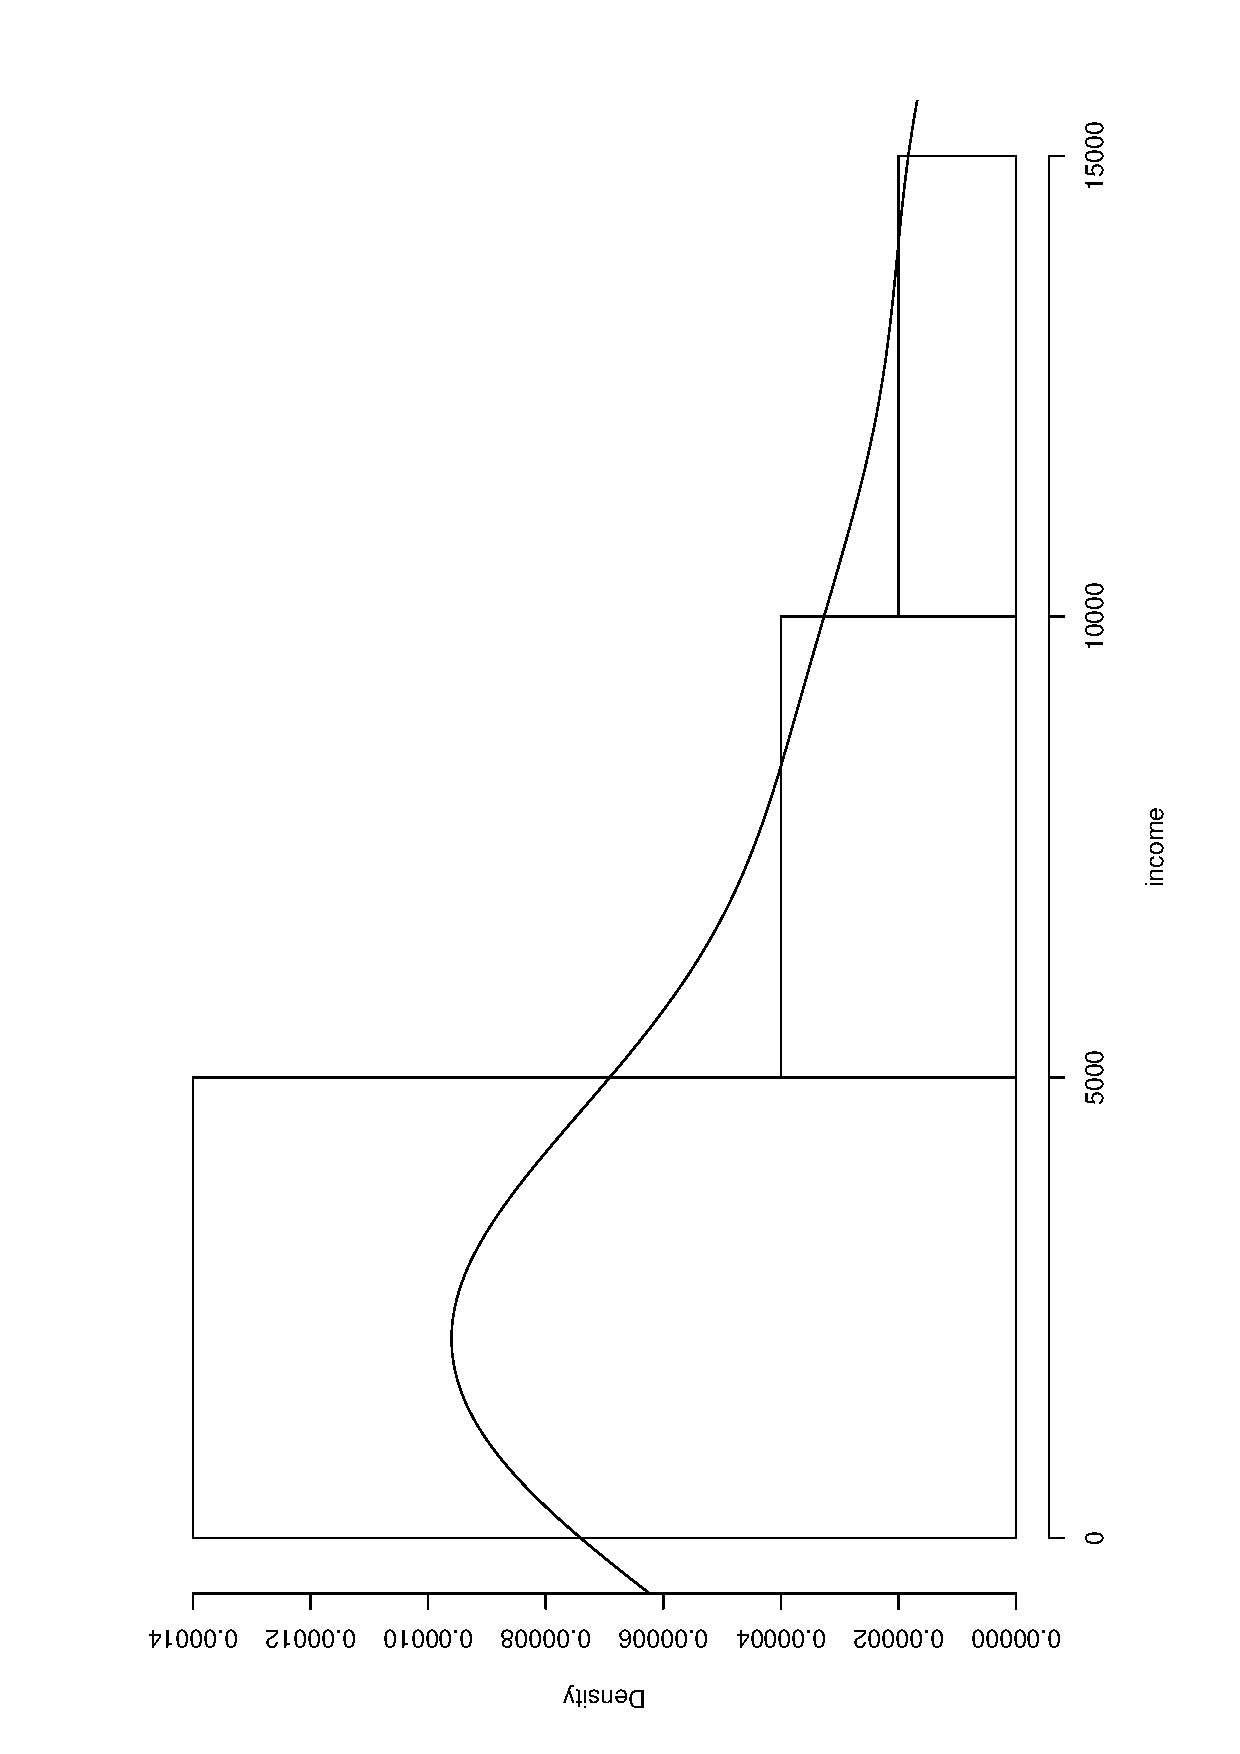
\includegraphics[scale=0.3, angle=90]{images/incomerhist.pdf}
%end{latexonly}
\htmlonly{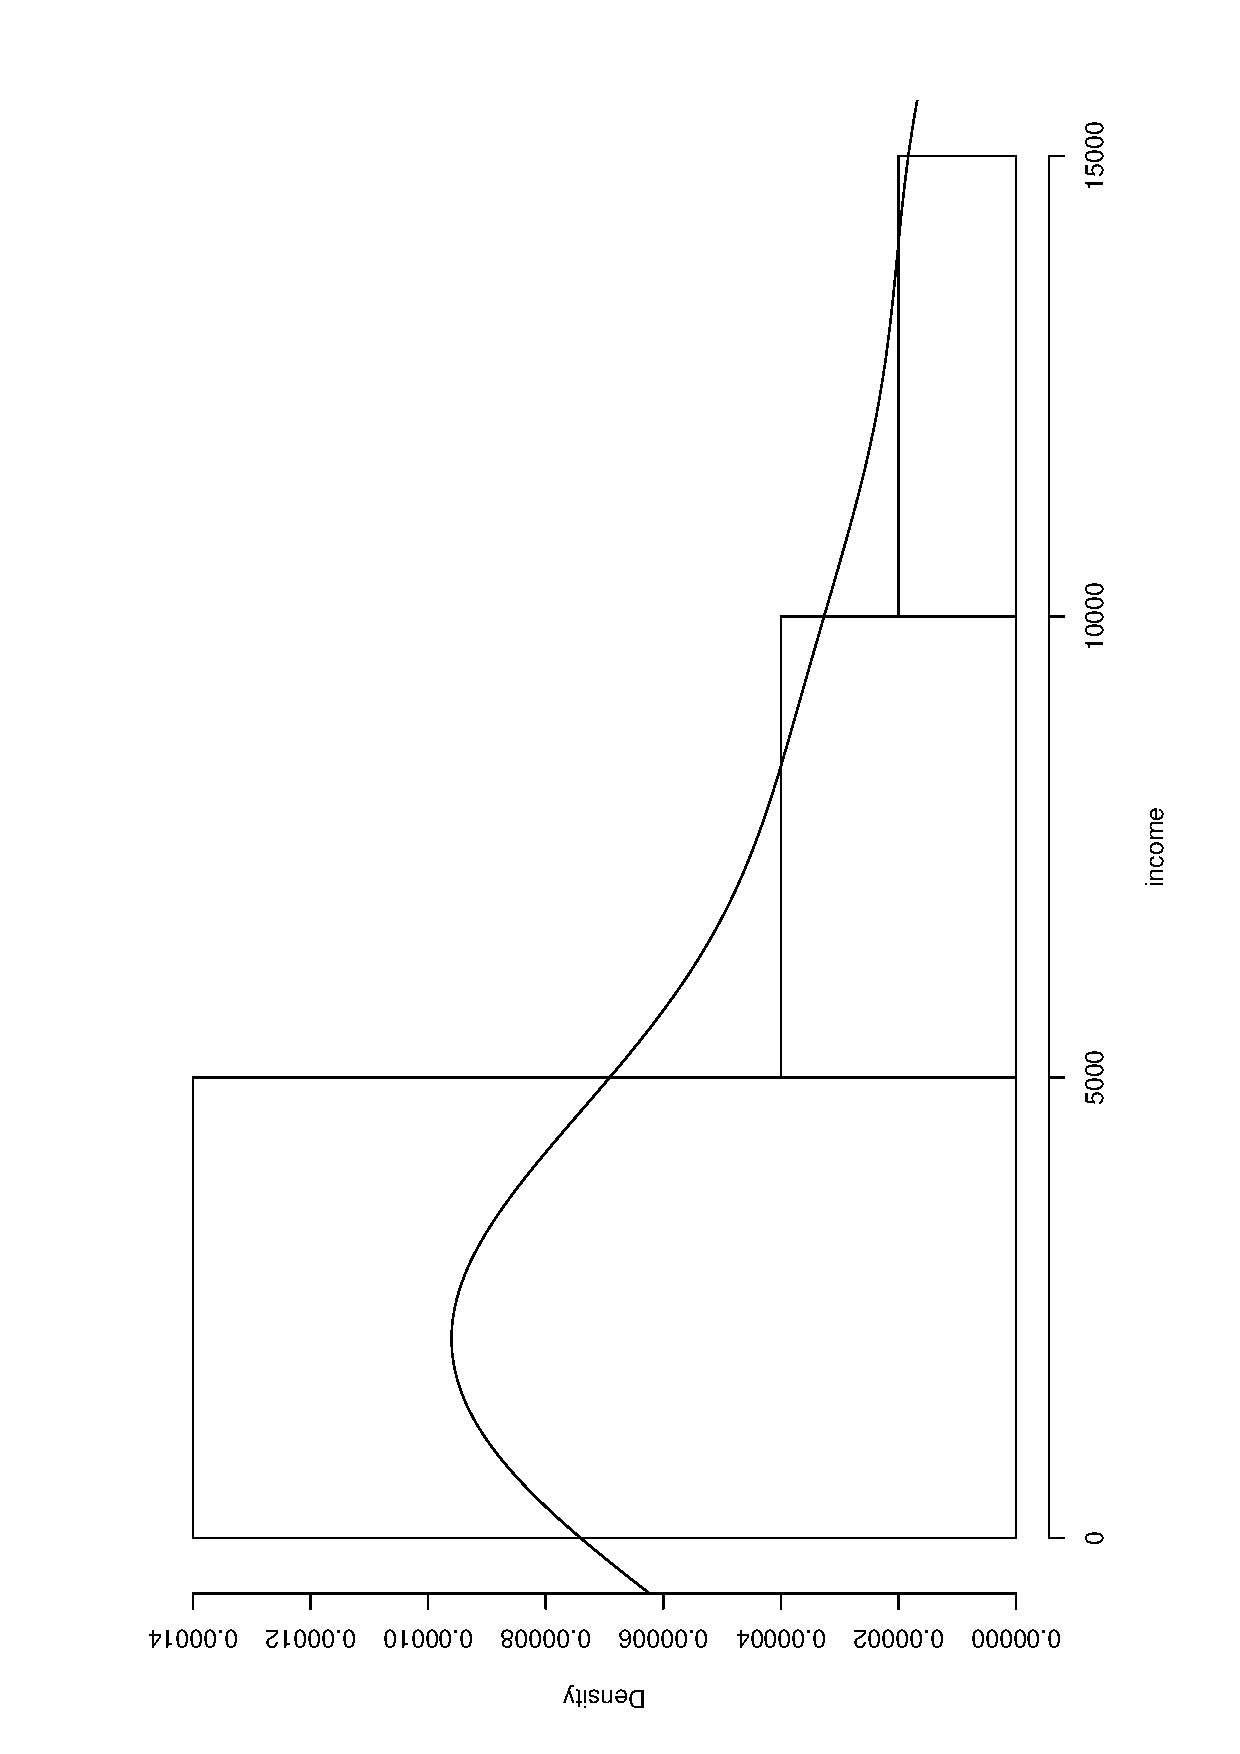
\includegraphics[scale=0.3, angle=90]{images/incomerhist.jpg}}
\end{center}

We can investigate a correlation \index{correlation} between attributes \attributesindex by plotting a scatter
plot \scatterplotindex (\module{rpy} \rpyindex library required):
\scatterplotindex
\begin{verbatim}
>>> households.r_scatter("persons", "income")
\end{verbatim}
\begin{center}
%begin{latexonly}
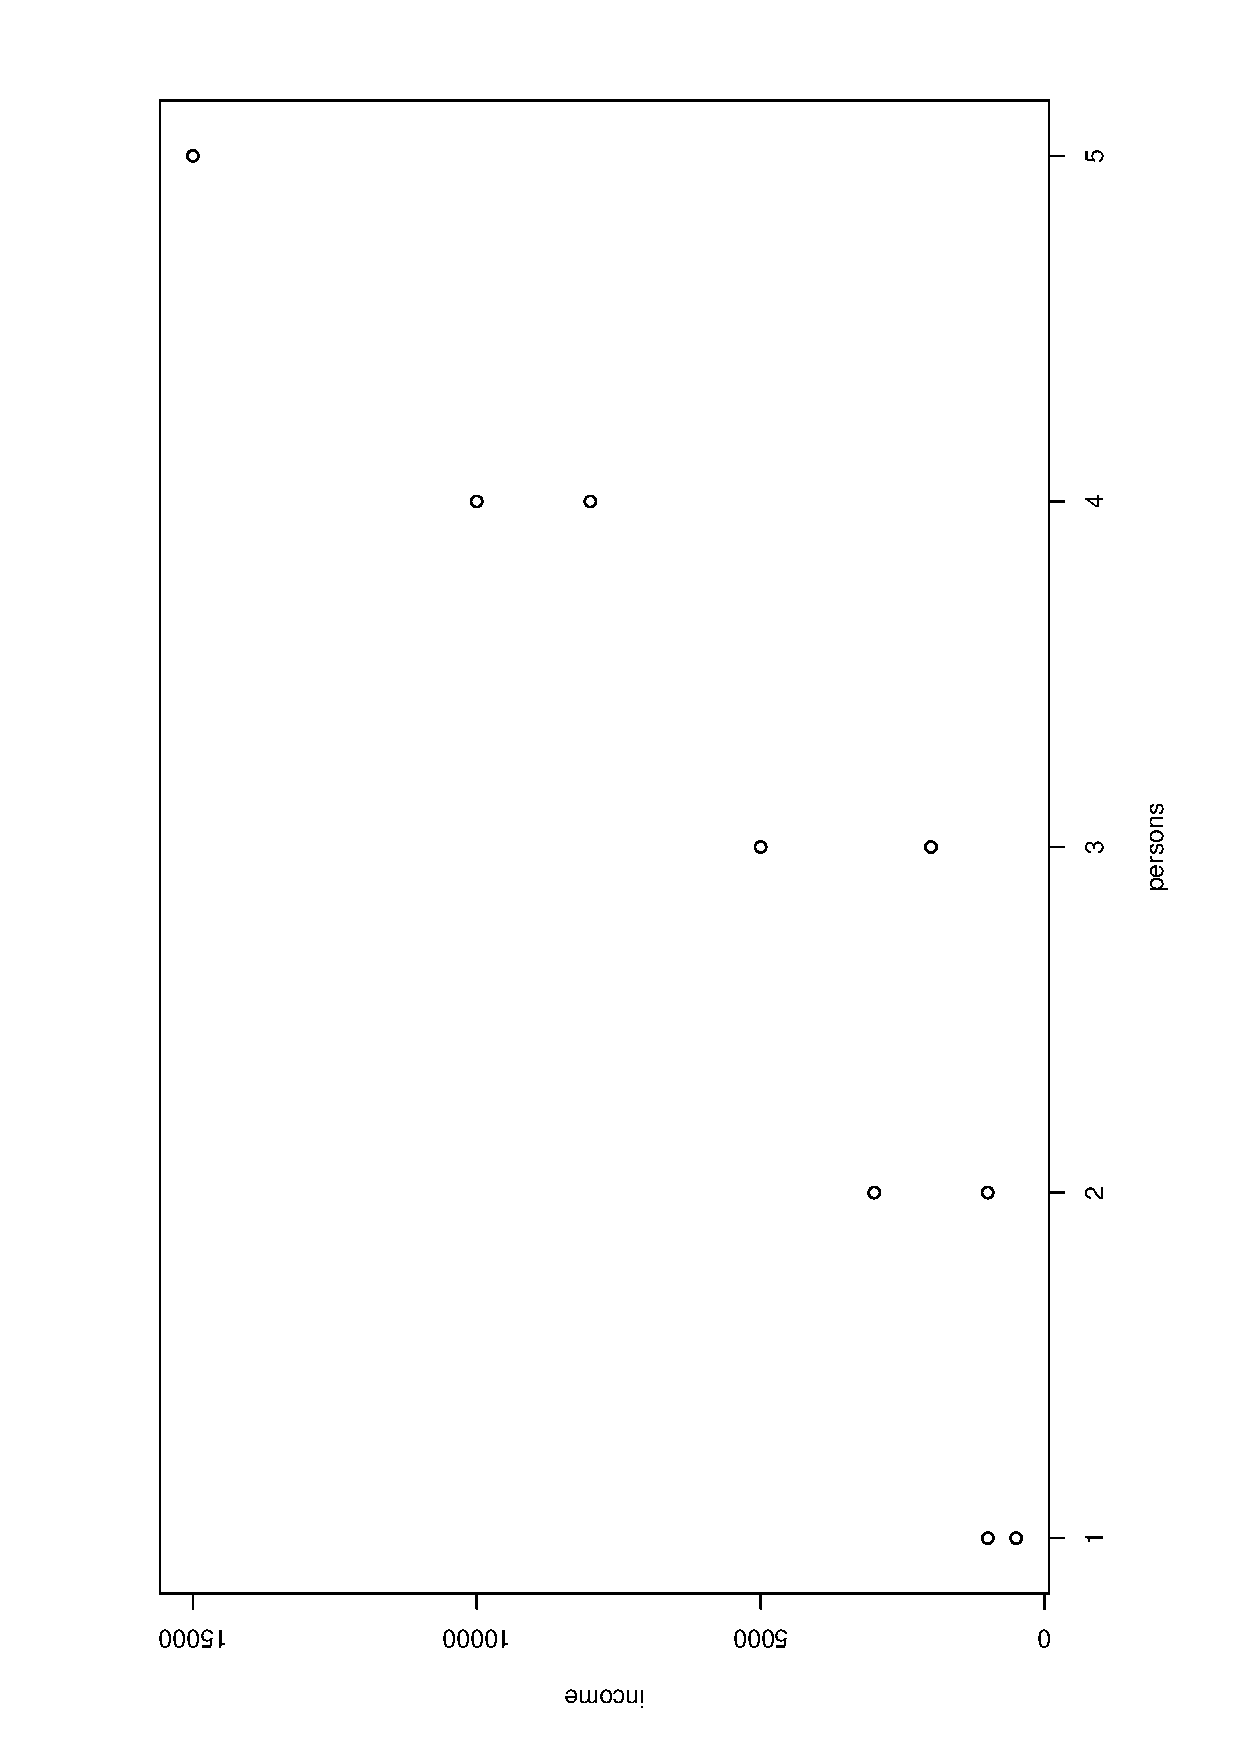
\includegraphics[scale=0.3, angle=90]{images/incomerscatter.pdf}
%end{latexonly}
\htmlonly{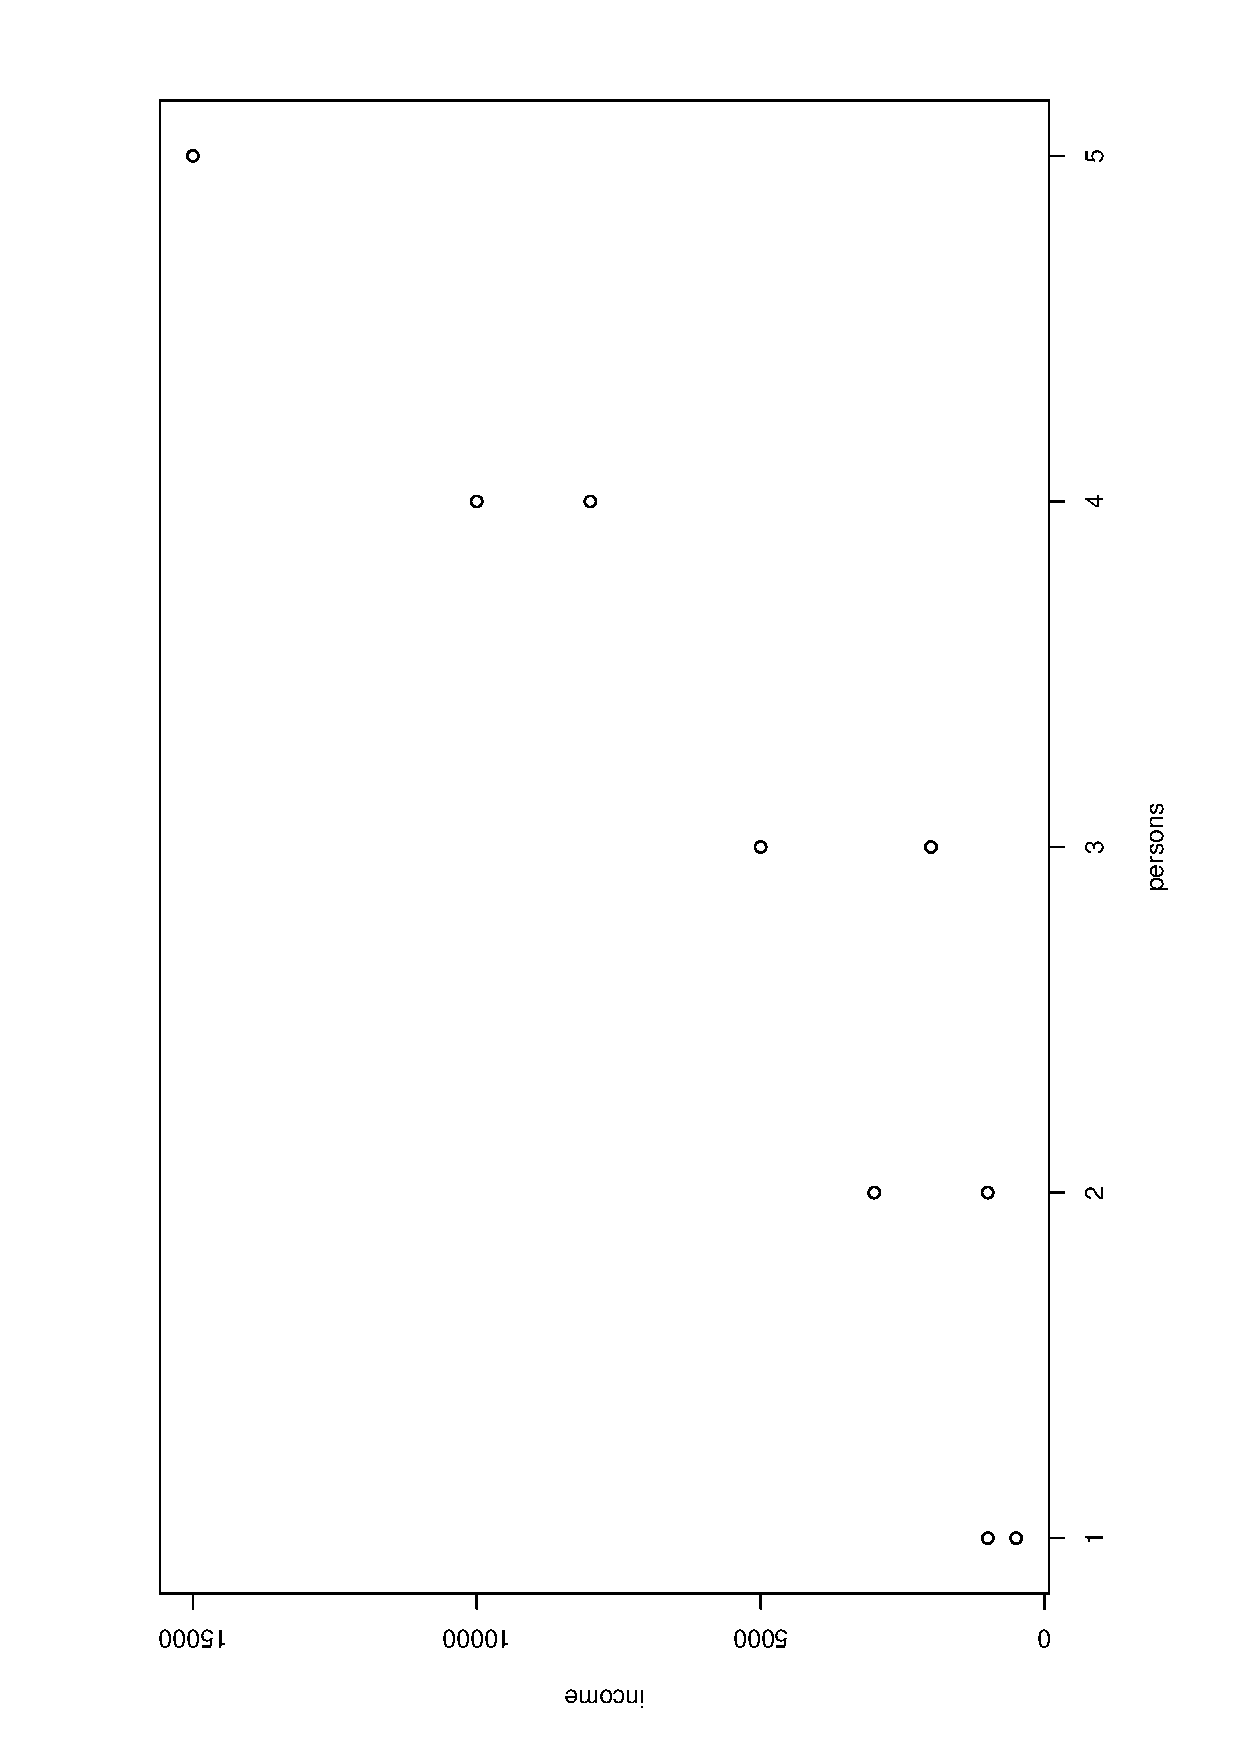
\includegraphics[scale=0.3, angle=90]{images/incomerscatter.jpg}}
\end{center}
\coefficientsindex
\begin{verbatim}
Correlation coefficient:  0.919147133827
\end{verbatim}

The correlation coefficient between two attributes and the correlation matrix of several attributes, respectively,
can be obtained by:
\begin{verbatim}
>>> households.correlation_coefficient("persons", "income")
0.91914713382720947
>>> households.correlation_matrix(["persons", "income"])
array([[ 1.        ,  0.91914713],
       [ 0.91914713,  1.        ]], type=float32)
\end{verbatim}

A summary of data in a dataset \datasetindex can by given by:

\attributesindex
\begin{verbatim}
>>> households.summary()
Attribute name        mean           sd           sum        min     max
-------------------------------------------------------------------------
        income      4850.0      4749.56         48500        500   15000
       persons         2.7         1.34            27          1       5


Size: 10  records
identifiers:
        household_id  in range  1 - 10
\end{verbatim}

To add an attribute \attributesindex to the set of households, for example each
household location, we do
\begin{verbatim}
>>> households.add_primary_attribute(data=[4,6,9,2,4,8,2,1,3,2], name="location")
>>> households.get_attribute_names()
['household_id', 'persons', 'location', 'income']
\end{verbatim}
If the attribute \attributesindex "location" already exists in the dataset, \datasetindex the values are
overwritten.

To change specific values in a dataset, \datasetindex one can use

\attributesindex
\begin{verbatim}
>>> households.modify_attribute(name="location", data=[0,0], index=[0,1])
>>> households.get_attribute("location")
array([0, 0, 9, 2, 4, 8, 2, 1, 3, 2])
\end{verbatim}
Here the argument \verb|index| determines the index of the data that are
modified.

To determine the location of household with \verb|household_id| $= 5$,
do
\begin{verbatim}
>>> households.get_data_element_by_id(5).location
4
\end{verbatim}

In order to store data in one of the supported formats,
you can use the {\tt storage} object created at the beginning of this section, or create a new one using
different directory/database:

\datasetindex
\begin{verbatim}
>>> households.write_dataset(out_storage=storage,
                             out_table_name="households_output")
\end{verbatim}

  Each dataset \datasetindex
  should have a unique dataset \datasetindex name that is used as an identification in
  variable \variablesindex computation (see
  Section~\ref{sec:variable-names}).

\begin{verbatim}
>>> households.get_dataset_name()
'household'
\end{verbatim}

{\it Here come more examples on variables and expressions}.
